\documentclass[14pt]{extreport}
\usepackage{amsmath}
\usepackage{amssymb}
\usepackage{float}
\usepackage[a4paper, total={7in, 10in}]{geometry}
\usepackage{graphicx}
\usepackage[utf8]{inputenc}

\title{
    NYU Tandon Bridge Spring 2022 \\
    Homework 4
}
\author{
    Cangyuan Li (Net ID: cl4220) \\
    Rishie Nandhan Babu (Net ID: rb5291) \\
    Amulya Thota        (Net ID: ast9920) \\
    Daniel Lim          (Net ID: dl3009)
}
\date{\today}

\newcommand{\homework}[9]{
	\noindent
	\begin{center}
		\framebox{
			\vbox{
				\hbox to 6.50in { {\bf NYU Computer Science Bridge to Tandon Course} \hfill Spring 2022 }
				\vspace{4mm}
				\hbox to 6.50in { {\Large \hfill Homework 4  \hfill} }
				\vspace{3mm}
				\hbox to 6.50in { \underline{Name(s)} \hfill \hspace{17mm} \underline{NetID(s)} \hfill \hfill }
				\vspace{2mm}
				\hbox to 6.50in { {#2} \hfill \hspace{15mm}{#3} \hfill \hfill \hfill \hfill \hfill }
				\hbox to 6.50in { {#4} \hfill \hspace{24mm}{#5}  \hfill \hfill \hfill }
				\hbox to 6in { {#6} \hfill \hspace{35mm}{#7} \hfill \hfill \hfill }
				\hbox to 6.50in { {#8} \hfill \hspace{31mm}{#9}  \hfill \hfill \hfill}
			}
		}
	\end{center}
	\vspace*{4mm}
}

\newcommand{\ddfrac}[2]{\frac{\displaystyle #1}{\displaystyle #2}}
\newcommand{\eq}[0]{\llap{\( \Leftrightarrow \) \qquad}}
\newcommand{\answer}[0]{\medskip \textbf{Answer:} \medskip}
\newcommand{\union}[0]{\cup}
\newcommand{\intersect}[0]{\cap}
\newcommand{\sumn}[0]{\( \sum\limits_{i=1}^n \)}
\newcommand{\limn}[0]{\( \lim_{n \to \infty} \)}
\newcommand{\limt}[0]{\( \lim_{t \to \infty} \)}
\newcommand{\R}[0]{\mathbb{R}}
\newcommand{\Z}[0]{\mathbb{Z}}

\begin{document}

\homework{1}{Rishie Nandhan Babu}{rb5291@nyu.edu}{Amulya Thota}{ast9920@nyu.edu}{Cangyuan Li}{cl4220@stern.nyu.edu}{Daniel Lim}{dl3009@nyu.edu}
\newpage

\section*{Question 9:}

\subsubsection*{Section A: zyBooks Exercise 4.1.3; b-c}

Which of the following functions are from \( \mathbb{R} \) to \( \mathbb{R} \)? If \( f \) is a function, give its range.

\begin{enumerate}
    \item[(b)] \( f(x) = \ddfrac{1}{x^2 - 4} \)
    
        \answer

        This is not a function from \( \R \) to \( \R \) because for \( x = 2 \) or \( x = -2 \), there is no corresponding \( y \).
    
    \item[(c)] \( f(x) = \sqrt{x^2} \)
    
        \answer

        This is a function from \( \R \) to \( \R \) because the square root is undefined only for negative numbers, and \( \forall x, x^2 >= 0 \). \( f \) is a function because there is exactly one \( y \) that corresponds to an \( x \). The range is \( [0, \infty) \) since \( \forall x, f(x) >= 0 \).

\end{enumerate}

\subsubsection*{Section B: zyBooks Exercise 4.1.5; b, d, h, i, l}

\begin{enumerate}
    
    \item[(b)] Let \( A = \left\{ 2, 3, 4, 5 \right\} \). \( f: A \rightarrow \Z \text{ s.t. } f(x) = x^2 \)
    
        \answer

        \{ 4, 9, 16, 25 \}
    
    \item[(d)] Let \( f: \{0, 1\}^{5} \rightarrow \Z \). For \( x \in \{ 0, 1 \}^5, f(x) \) is the number of 1's that occur in \( x \).

        \answer

        The range is \{ 0, 1, 2, 3, 4, 5 \}. There can be at most 5 1's in a string 11111, and the lowest possible is 0 1's in a string 00000.

    \item[(h)] Let \( A = \left\{ 1, 2, 3 \right\} \). \( f: A \times A \rightarrow \Z \times \Z \), where \( f(x, y) = (y, x) \)
    
        \answer

        Step 1: \( A \times A = \left\{ (1, 1), (1, 2), (1, 3), (2, 1), (2, 2), (2, 3), (3, 1), (3, 2), (3, 3) \right\} \)

        \medskip

        Step 2: Since \( A = A \), \( (x, y) = (y, x) \), so the range is the set in Step 1.

    \item[(i)] Let \( A = \left\{ 1, 2, 3 \right\} \). \( f: A \times A \rightarrow \Z \times \Z \), where \( f(x, y) = (x, y + 1) \)
    
        \answer

        From (h) we have \( A \times A = \left\{ (1, 1), (1, 2), (1, 3), (2, 1), (2, 2), (2, 3), (3, 1), (3, 2), (3, 3) \right\} \). Then the range is:
        \[
            \left\{ (1, 2), (1, 3), (1, 4), (2, 2), (2, 3), (2, 4), (3, 2), (3, 3), (3, 4) \right\}
        \]

    \item[(l)] Let \( A = \left\{ 1, 2, 3 \right\} \). \( f: \mathcal{P}(A) \rightarrow \mathcal{P}(A) \). For \( X \subseteq A, f(X) = X - \{1\} \)
    
        \answer

        Step 1: \( \mathcal{P}(A) = \left\{ \varnothing, \{ 1 \}, \{ 2 \}, \{ 3 \}, \{ 1, 2 \}, \{ 1, 3 \}, \{ 2, 3 \}, \{ 1, 2, 3 \} \right\} \)

        \medskip

        Step 2: All elements of the powerset are by definition subsets of \( A \), so the range is:
        \[
            \left\{ \varnothing, \{ 2 \}, \{ 3 \}, \{ 2, 3 \} \right\} 
        \]
        
\end{enumerate}
\newpage

\section*{Question 10:}

\subsection*{Part I.}

\subsubsection*{Section A: zyBooks Exercise 4.2.2; c, g, k}
    
Indicate if the function is one-to-one or not, and if it is onto or not. If not one-to-one or onto, give an example showing why. 

\begin{enumerate}
    \item[(c)] $f: \textbf{Z} \to \textbf{Z}. \hspace{2mm} h(x) = x^{3}$
    
        \answer

            One-to-one, but not Onto.
            
            One-to-one: no two integers have the same result when the raised to the power 3. 
            
            Not onto: there are examples for $y$ in target set for which there is no $x$ in the domain such that $x^{3} = y$. For example: 2, 3, 4 etc have no integer cube roots.
    \newline
    \item[(g)] $f: \textbf{Z}\hspace{1mm} X \hspace{1mm}\textbf{Z} \to \textbf{Z} X \textbf{Z}. \hspace{2mm} f(x,y) = (x+1, 2y)$
    
        \answer
        One-to-one, but not Onto. 
        
        One-to-one: no two elements of the domain can be mapped to the same element in the target. 
        
        Not onto: for example , for $\left(2,3\right)$ in the Target, there is no corresponding $\left(x,y\right)$ in the Domain as there is no y such that $2y = 3$. 
    \newline
    
    \item[(k)] $f: \textbf{Z} ^{+} \to \textbf{Z} ^{+}$.\hspace{1mm} $f(x,y) = 2^{x} + y$
    
        \answer
        Neither one-to-one or onto. 
        
        Not one-to-one: Example: Let us consider the integer 7 in the target. For two elements in the Domain $\left(1,5\right)$ and $\left(2,3\right)$, the function maps to 7 in the Target. 
        
        Not onto: Example: For integer 1 in the target, there is no $\left(x,y\right)$ in the Domain such that the function maps it to 1 in the Target. 

\end{enumerate}

\subsubsection*{Section B: zyBooks Exercise 4.2.4; b, c, d, g}

Indicate if the function is one-to-one, onto, neither, or both. If not one-to-one or onto, give an example showing why.
    
\begin{enumerate}
    
    \item[(b)] $f\{0,1\}^{3} \to \{0,1\}^{3}$
    
        \answer

        Neither one-to-one nor Onto
        
        Not one-to-one: For example, two elements of the domain: 000 and 100 are mapped to the same element 100 in the target. \\
        $f\left(000\right) = f\left(100\right) = 100$
        \newline
        Not onto: For example, the element (000) in the Target does not have a corresponding element in the domain.
        \newline

    \item[(c)] $f\{0,1\}^{3} \to \{0,1\}^{3}$ : The output of f is obtained by taking the input string and reversing the bits.
    
        \answer

        Both one-to-one and onto.
        
        One-to-one: Since each element in the domain is unique, its reverse, i.e, the corresponding element in the Target is also unique.   
        
        Onto: Every element in the target can be identified as a reverse of an element in the domain.  
        \newline

    \item[(d)] $f\{0,1\}^{3} \to \{0,1\}^{4}$ : The output of f is obtained by taking the input string and adding an extra copy of the first bit to the end of the string.
    
        \answer

        One-to-one, but not Onto. 
        
        One-to-one: every element in the domain has a unique corresponding element in the target. 
        
        Not onto: The elements the target that have non-identical first and last bits: such as 0001
        \newpage
        
    \item[(g)] Let A be defined as the set \{1,2,3,4,5,6,7,8\} and B be defined as \{1\}. \\
    \(f: P\left(A\right) \to P\left(A\right)\). For \(X \subseteq A\), \(f\left(X\right) = X-B\)
    
        \answer
        
        Neither One-to-one nor Onto. \\
        
        Not one-to-one: \\
        Example: Consider these two subsets of A \(\{2\} and \{1,2\}\). \\Since \(f\left(X\right) = X-B\), 
        \newline
        \(f\{2\} = \{2\}-\{1\} = \{2\}\) \\
        \(f\{1,2\} = \{1,2\}-\{1\} = \{2\}\) \\
        Both \(\{2\} and \{1,2\}\) in the Domain set map to the same corresponding element \(\{2\}\) in the Target set. Hence not one-to-one. 
        \newline
        
        Not onto: \\
        Example : Consider \(\{1\}\) in the target set. There is no corresponding X in the Domain set such that \(f\left(X\right) = \{1\}\). Hence, not onto. 
        
\end{enumerate}

\subsection*{Part II.}

Give an example of a function from the set of integers to the set of positive integers ($\mathbb{Z} \rightarrow \mathbb{Z^{+}}$) that is: 

\begin{enumerate}
    \item[(a)] One-to-one, but not onto. 
        
        $f(x) = \begin{cases} \text{if x is negative,} & |x| \cdot 2 \\ \text{if x is non-negative,} & 2x+3 \end{cases}  $
        
        If $x$ is negative, $f(x)$ will always be positive and even. \\
        If $x$ is positive, the lowest possible $f(x)$ is 5. \\
        If $x$ is zero, $f(x)$ is 3. \\
        All non-negative $x$ outputs an odd/positive $f(x)$. \\
        But there is no $x$ such that $f(x) = 1$ . \\
        $\therefore$ \text{One-to-one, but not onto.} 
        \newline
        
        \item[(b)] Onto, but not one-to-one. 
        
        $f(x) = |x|+1$
        
        Not one-to-one because $x=2 and x=-2$ can produce the same $f(x) = 3$. \\
        Onto, because for every $f(x)$ value, there exists some corresponding $x$ that outputs it. \\
        $\therefore$ \text{Onto, but not one-to-one.} 
        \newline
        
        \item[(c)] One-to-one and onto. 
        
        $f(x) = \begin{cases} \text{if x is negative,} & |x| \cdot 2 \\ \text{if x is non-negative,} & 2x+1 \end{cases}  $
        
        If $x$ is 0, $f(x) = 1$\\
        If $x$ is positive, $f(x) = 3, 5, 7, ...$ (all positive odd integers)\\
        If $x$ is negative, $f(x) = 2, 4, 6, ...$ (all positive even integers)\\
        $\therefore$ One-to-one and onto (bijection).
        \newline
        
        \item[(d)] Neither one-to-one nor onto. 
        
        $f(x) = x^2 +1$
        If $x=-1 \text{ or } 1$, then $f(x) = 2$ for either. Hence, not one-to-one.\\ 
        Considering the case where $f(x) = 7 \text{ or } 11$ or any other positive integer that is not a perfect square +1, there does not exist an integer solution of $x$. \\
        $\therefore$ Neither one-to-one nor onto. 
\end{enumerate}
\newpage

\section*{Question 11:}

\subsubsection*{zyBooks Exercise 4.3.2; c, d, g, i.}
    
For each of the following functions, indicate whether the function has a well-defined inverse. If the inverse is well-defined, give the input/output relationship of $f^{-1}$.
    
\begin{enumerate}
    \item[(c)] $f: \mathbb{R} \to \mathbb{R}. \hspace{2mm} f(x) = 2x+3$
    
        \answer

        $\Rightarrow$ Both one-to-one and onto, so the function has a well-defined inverse. \\
        $\Rightarrow$ Let $f(x)=y$, so $y=2x+3$\\
        $\Rightarrow$ $2x=y-3$\\
        $\Rightarrow$ $x=\frac{y-3}{2}$\\
        $\therefore$ $f^{-1}(y) = \frac{y-3}{2}$.
        \newline
    
    \item[(d)] Let $A$ be defined to be the set $\{1,2,3,4,5,6,7,8\}$ \\
    $f: P(A) \rightarrow \{0,1,2,3,4,5,6,7,8\}$ \\
    For $X \subseteq A, f(x) = |X|$. Recall that for a finite set $A, P(A)$ denotes the power set of $A$ which is the set of all subsets of $A$.
    
        \answer

        $\Rightarrow$ Not one to one, as $f(\{1\})$ and $f(\{2\})$ have the same cardinality of $f(x) = |X| = 1$. \\
        $\Rightarrow$ Not onto, since there is no $X \subseteq P(A)$ that has a cardinality of 0. The smallest $|X| =1$, for $\{1\}$ or $\emptyset$ \\
        $\therefore$ Well-defined inverse does not exist.
        \newline
        
    \item[(g)] $f:\{0,1\}^3 \rightarrow f:\{0,1\}^3$. The output of $f$ is obtained by taking the input string and replacing the first bit by 1, regardless of whetehr the first bit is a 0 or 1. For example, $f(001) = 101$ and $f(110) = 110.$
        
        \answer
        
        $\Rightarrow$ Function is both one-to-one and onto, and hence has a well-defined inverse.\\
        $\Rightarrow$ $f^{-1}(x) =$ The inverse output is obtained by simply taking the input string and reversing, which is the same as the function itself.\\
        $\therefore$ $f^{-1} = f$.
        \newline
        \\
        \\
        \\
        
        
    \item[(i)] $f:\mathbb{Z} \times \mathbb{Z} \rightarrow \mathbb{Z} \times \mathbb{Z}, f(x,y) = (x+5, y-2)$. 
        
        \answer
        
        $\Rightarrow$ Function is both one-to-one and onto, and hence has a well-defined inverse.\\
        $\Rightarrow$ Let $f(x,y)$ be $P,Q$, so $P=x+5$ and $Q=y-2$\\
        $\Rightarrow$ Solve for $x, y$ with respect to $P, Q$\\
        $\Rightarrow$ So $x=P-5$, $y=Q+2$\\
        $\therefore$ $f^{-1}(x,y) = (x-5, y+2)$. 
        \newline
\end{enumerate}
    
\subsubsection*{Section B: zyBooks Exercise 4.4.8; c, d}

The domain and target set of functions f, g, and h are $\mathbb{Z}$. The functions are defined as: 
\begin{itemize}
    \item $f(x) = 2x+3$
    \item $g(x) = 5x+7$
    \item$h(x) = x^2+1$
\end{itemize}
    
\begin{enumerate}
    \item[(c)] $f \circ h$
    
        \answer
        \begin{align*}
            f(h(x)) &= 2(x^2+1)+3\\
                    &= 2x^2 +2+3\\
                    &=2x^2+5
        \end{align*}
        
    \item[(d)] $h \circ f$
        
        \answer
        \begin{align*}
            h(f(x)) &= (2x+3)^2 +1\\
                    &= (2x)^2 +2 \cdot 2x \cdot 3 + 3^2 +1\\
                    &= 4x^2 + 12 x + 10
        \end{align*}
        
\end{enumerate}

\subsubsection*{Section C: zyBooks Exercise 4.4.2; b-d}

\begin{enumerate}

    \item[(b)]
    
        \answer

        \begin{align*}
            \left ( f \circ h \right )\left ( x \right ) = f\left ( h\left ( x \right ) \right ) \\
            = f\left (  \left \lceil \frac{x}{5} \right \rceil \right ) \\
            = \left (  \left \lceil \frac{x}{5} \right \rceil \right )^{2} \\\\
            \therefore \left ( f \circ h \right )\left ( 52 \right ) = \left (  \left \lceil \frac{52}{5} \right \rceil \right )^{2} \\
            = \left ( \left \lceil 10.4 \right \rceil \right )^{2} \\
            = \left ( 11 \right )^{2} = 121
        \end{align*}

    \item[(c)]
    
        \answer

        \begin{align*}
            \left ( g \circ h \circ f \right )\left ( x \right ) = g\left ( h\left ( f\left ( x \right ) \right ) \right ) \\
            = g\left ( h\left ( x^{2} \right ) \right ) \\
            = g\left (  \left \lceil \frac{x^2}{5} \right \rceil \right ) \\
            = 2^{\left \lceil \frac{x^2}{5} \right \rceil} \\\\
            \therefore \left ( g \circ h \circ f \right )\left ( 4 \right ) = 2^{\left \lceil \frac{16}{5} \right \rceil} \\
            = 2^{4} \\
            = 16
        \end{align*}

    \item[(d)]
    
        \answer

        \begin{align*}
            \left ( h \circ f \right )\left ( x \right ) = h\left ( f\left ( x \right ) \right ) \\
            = h\left ( x^{2} \right ) \\
            = \left \lceil \frac{x^{2}}{5} \right \rceil
        \end{align*}

\end{enumerate}
\newpage

\subsubsection*{Section D: zyBooks Exercise 4.4.6; c-e}

Define the following functions \( f \), \( g \), and \( h \):

\begin{itemize}
    \item \( f: \{0, 1\}^3 \rightarrow \{0, 1\}^3 \). The output of \( f \) is obtained by taking the input string and replacing the first bit by 1, regardless of whether the first bit is a 0 or 1.
    \item \( g: \{0, 1\}^3 \rightarrow \{0, 1\}^3 \). The output of \( g \) is obtained by taking the input string and reversing the bits.
    \item \( h: \{0, 1\}^3 \rightarrow \{0, 1\}^3 \). The output of \( h \) is obtained by taking the input string \( x \), and replacing the last bit with a copy of the first bit.
\end{itemize}
	
\begin{enumerate}
    \item[(c)] What is \( (h \circ f)(010) \)?
    
        \answer

        \begin{align*}
            \left ( h \circ f \right )\left ( 010 \right ) = h\left ( f\left ( 010 \right ) \right ) \\
            = h(110) \\
            = 111
        \end{align*}

    \item[(d)] What is the range of \( h \circ f \)?
    
        \answer

        \begin{table}[H]
            \centering
            \hspace{20mm}
            \begin{tabular}{lll}
            Domain & f(x) & h(f(x)) \\ \hline
            000    & 100  & 101     \\
            001    & 101  & 101     \\
            010    & 110  & 111     \\
            011    & 111  & 111     \\
            100    & 100  & 101     \\
            101    & 101  & 101     \\
            110    & 110  & 111     \\
            111    & 111  & 111    
            \end{tabular}
        \end{table}

        $\therefore$ Range of $h \circ f = \left \{ 101, 111 \right \}$
        \newpage

    \item[(e)] What is the range of \( g \circ f \)?
    
        \answer
    
        \begin{table}[H]
            \centering
            \hspace{20mm}
            \begin{tabular}{lll}
            Domain & f(x) & g(f(x)) \\ \hline
            000    & 100  & 001     \\
            001    & 101  & 101     \\
            010    & 110  & 011     \\
            011    & 111  & 111     \\
            100    & 100  & 001     \\
            101    & 101  & 101     \\
            110    & 110  & 011     \\
            111    & 111  & 111    
            \end{tabular}
        \end{table}

        $\therefore$ Range of $g \circ f = \left \{ 001, 101, 011, 111 \right \}$

\end{enumerate}
	
\subsubsection*{Section E: Extra Credit, zyBooks Exercise 4.4.4; c, d}

Let \( f: X \rightarrow Y \) and \( g: Y \rightarrow X \) be two functions.
	
\begin{enumerate}

    \item[(c)] Is it possible that \( f \) is not one-to-one and \( g \circ f \) is one-to-one? Justify your answer. If the answer is "yes", give a specific example for \( f \) and \( g \).
    
        \answer

        Let us assume $g \circ f$ is one-to-one. We will show that $f$ has to be one-to-one. \\\\
        Assume $x_{1} \in X, x_{2} \in X$ such that $x_{1} \neq x_{2}$. \\\\
        Since $\left ( g \circ f \right )\left ( x \right )$ is one-to-one,
        \begin{align*}
            g(f(x_{1})) \neq g(f(x_{2}))
        \end{align*}
        Taking inverse of $g$ on both sides, we get,
        \begin{align*}
            g^{-1}(g(f(x_1))) \neq g^{-1}(g(f(x_2)))\\
            \Rightarrow f(x_1) \neq f(x_2) \hspace{5mm}[as \hspace{2mm} h^{-1}(h(x)) = x]
        \end{align*}
        Hence, $f$ is one-to-one. \\\\
        i.e. If $g \circ f$ is one-to-one, we must have $f$ as one-to-one. $\blacksquare$ 

    \newpage
        
    \item[(d)] Is it possible that \( g \) is not one-to-one and \( g \circ f \) is one-to-one? Justify your answer. If the answer is "yes", give a specific example for \( f \) and \( g \).
    
        \answer
        
        Following example depicts that $g$ is not one-to-one and $g \circ f$ is one-to-one. \\
        \begin{figure}[htp]
            \centering
            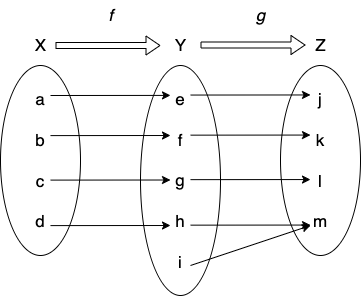
\includegraphics[width=10cm]{VennDiagramQ11.png}
        \end{figure}
    
\end{enumerate}
\newpage
	

\end{document}